In the previous Chapter, we explored the time evolution of a wave function governed by the evolution operator, $\hat{U}(t)$, and introduced a simple numerical technique for propagating the wave function. This way we can study dynamical processes governed by quantum mechanics and explore intricacies of the quantum world like interference or tunnelling. However, the time evolution of a wave function offers more than just insight into the system's dynamics -- it also encodes the energy spectrum of the system. Although counter-intuitive, we can obtain the energy spectrum, a time-independent quantity usually calculated by solving the \acrfull{tise}, by performing a dynamical simulation. This time-dependent perspective is widely used in theoretical spectroscopy where both the energy spectrum and intensities are calculated from quantum or semiclassical dynamics.

\section{Theoretical background}
\label{sec:autocorrintro}

To understand how the energy spectrum is encoded in the wave function propagation, we examine the exact solution of the \acrlong{tdse}. Assume we could solve the \acrshort{tise}
\begin{equation}
    \hat{H}(x) \phi_k(x) = E_k \phi_k(x)
    \label{eq:tise0}
\end{equation}
and obtain a complete set of eigenfunctions $\phi_k(x)$.\footnote{In practice, obtaining these eigenfunctions is often the most challenging step in this approach, as they cannot usually be computed directly. Therefore, this method is more useful for deriving theoretical insights rather than for practical calculations.} This set of eignefunctions forms an orthonormal basis, allowing us to expand any wave function as a linear combination of $\phi_k$. Expanding the initial wave function in this basis, we write:
\begin{equation}
    \psi(x,0) = \sum_k c_k \phi_k(x) \, ,
\end{equation}
where $c_k$ are the expansion coefficients determined as 
\begin{equation}
    c_k = \langle \phi_k(x) | \psi(x,0) \rangle = \int_{-\infty}^\infty \phi_k^*(x) \psi(x,0) \dd x \, .
    \label{eq:psi0v1}
\end{equation}

The solution of the \acrshort{tdse}, $\psi(x,t)$, can be calculated by applying the propagator $\hat{U}(t)$ to the initial wave function (Eqs.~\eqref{eq:U} and~\eqref{eq:U1}):
\begin{equation}
    \psi(x,t) = \hat{U}(t)\psi(x,0) = \e^{-\frac{i}{\hbar}\hat{H}(x)t} \psi(x,0) = \sum_k c_k \e^{-\frac{i}{\hbar}\hat{H}(x)t} \phi_k(x) \, .
\end{equation}
Since $\phi_k$ are eigenfunctions of the Hamiltonian $\hat{H}$, the propagator acts on each $\phi_k$ as:
\begin{equation}
    \e^{-\frac{i}{\hbar}\hat{H}(x)t} \phi_k(x) = \e^{-\frac{i}{\hbar}E_k t} \phi_k(x) \, ,
\end{equation}
leading to the time-dependent solution:
\begin{equation}
    \psi(x,t) = \sum_k c_k \e^{-\frac{i}{\hbar}E_k t}\phi_k(x) \, .
    \label{eq:tdpsi1}
\end{equation}
This expression represents the exact solution of the \acrshort{tdse} in the basis of Hamiltonian eigenstates. For time-independent Hamiltonians (i.e., $\hat{H} \neq \hat{H}(t)$), the coefficients $c_k$ remain constant over time, and the only time-dependent terms are the exponentials $\e^{-\frac{i}{\hbar}E_k t}$, fully governing the evolution.

Using this exact \acrshort{tdse} solution, we can now extract the energy spectrum through the \textit{autocorrelation function}. The autocorrelation function is defined as an overlap of the wave function at time $t$ with the initial wave function at time 0:
\begin{equation}
    S(t) = \langle \psi(x,0) | \psi(x,t) \rangle =\int_{-\infty}^{\infty}\psi^*(x,0) \psi(x,t) \dd x\, .
\end{equation}
It measures the probability amplitude of $\psi(x,t)$ being in the initial state $\psi(x,0)$. Thus, the autocorrelation function is always equal to 1 at time 0. Inserting the exact solution of \acrshort{tdse} \eqref{eq:tdpsi1}, the autocorrelation function reads
\begin{align}
    S(t) &= \int_{-\infty}^{\infty} \sum_l \sum_k c_l^* \phi_l^*(x) c_k \e^{-\frac{i}{\hbar}E_k t}\phi_k(x) \dd x \notag\\
    &= \sum_l \sum_k c^*_l c_k \e^{-\frac{i}{\hbar}E_k t} \int_{-\infty}^{\infty}  \phi_l^*(x) \phi_k(x) \dd x \notag\\
    &= \sum_l \sum_k c^*_l c_k \e^{-\frac{i}{\hbar}E_k t} \delta_{kl} \notag\\
    &= \sum_k |c_k|^2 \e^{-\frac{i}{\hbar}E_k t} \, .
\end{align}
It appears that the autocorrelation function is a sum of the time-dependent exponentials weighted by magnitudes of the coefficients $c_k$. The energy spectrum $\sigma$ can then be obtained by applying \acrshort{ift} to the autocorrelation function:
\begin{equation}
    \sigma(E) = \int_{-\infty}^{\infty} S(t) \e^{\frac{i}{\hbar}Et} \dd t  = \sum_k |c_k|^2 \int_{-\infty}^{\infty} \e^{\frac{i}{\hbar}(E-E_k)t} \dd t = \sum_k |c_k|^2 \delta(E-E_k) \, ,
    \label{eq:autocorr1}
\end{equation}
where the Dirac $\delta$-distributions are centred at energies $E_k$ with magnitudes $|c_k|^2$. Thus, the spectrum exhibits peaks at all eigenvalues $E_k$ for which $c_k\neq 0$ in the initial wave function $\psi(x,0)$, see Fig.~\ref{eq:autocorr1}.

\begin{figure}[ht!]
    \centering
    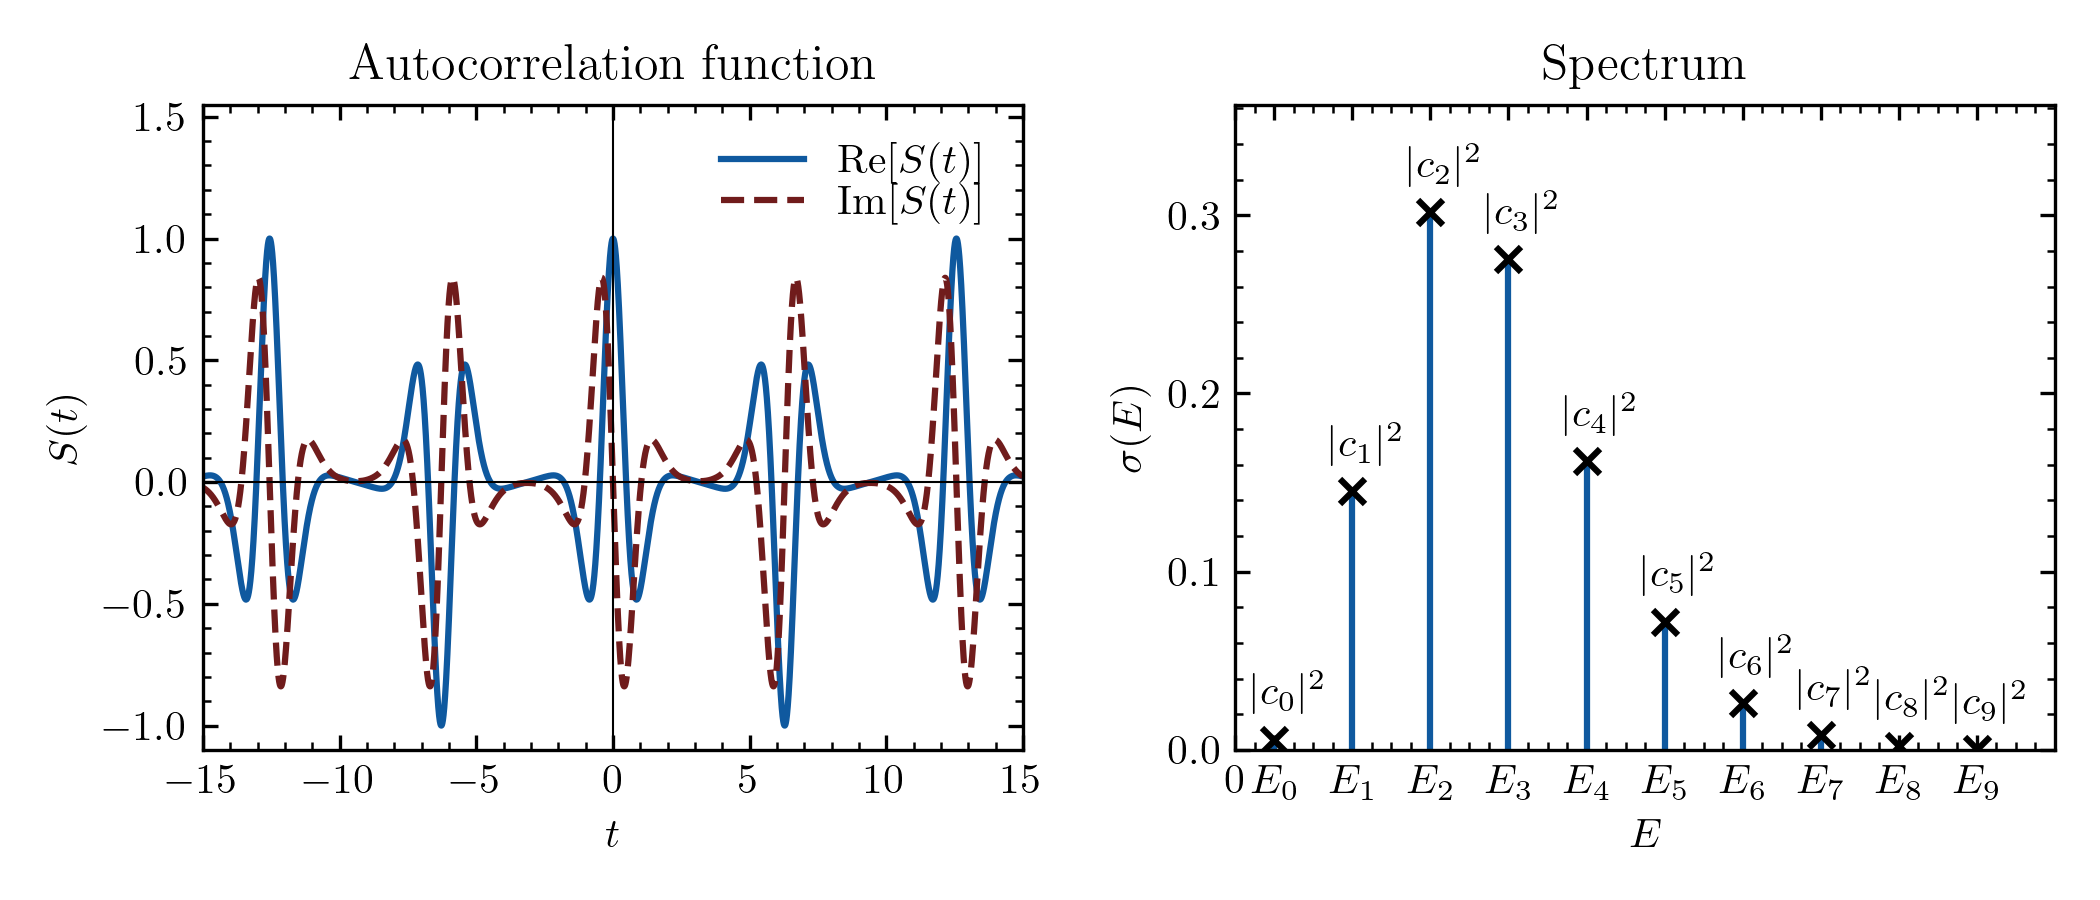
\includegraphics[width=0.9\linewidth]{scriptum/obrazky/autocorr/autocorr1.png}
    \caption{An illustrative example of autocorrelation function $S(t)$ of a harmonic oscillator (left) and its corresponding energy spectrum $\sigma(E)$ (right).}
    \label{fig:autocorr1}
\end{figure}

Although this analysis is based on the exact TDSE solution and the full set of eigenfunctions $\phi_k$, the derived autocorrelation function $S(t)$ and energy spectrum $\sigma(E)$ apply to any wave function evolution. This method provides a powerful tool for calculating the spectrum of any Hamiltonian by time-propagating a wave function, which is often computationally more feasible than directly diagonalizing the Hamiltonian.

\section{*Numerical application}
\label{sec:autocorr_numap}

The numerical implementation of the outlined procedure is straightforward in this case. We need to \acrlong{ift} the autocorrelation function $S(t)$, which is a simple overlap between $\psi(x,t)$ and $\psi(x,0)$. As we have shown in Chapter~\ref{kap:qd}, there are readily available numerical techniques to calculate \acrlong{ift} and overlaps. However, we face another difficulty in this case. Typically, we propagate the wave function for time 0 to some finite time $t$ in our simulation. However, the integral in the \acrlong{ift} in Eq.~\eqref{eq:autocorr1} runs from time $-\infty$ to $\infty$ which requires the knowledge of the autocorrelation function from time $-\infty$ to $\infty$. Thus, we have two problems: we have no information about $S(t)$ in the negative times and we have information about $S(t)$ in the positive times only to some maximum time $t_\mathrm{max}$.

The first problem can be addressed but exploring the properties of the autocorrelation function:
\begin{align}
    S^*(t) &= \langle \psi(x,0) | \psi(x,t) \rangle^* = \langle \psi(x,0) | \e^{-\frac{i}{\hbar}\hat{H}(x)t} |\psi(x,0) \rangle^* = \langle \psi(x,0) | \e^{\frac{i}{\hbar}\hat{H}(x)t} |\psi(x,0) \rangle \notag \\
    &= \langle \psi(x,0) | \e^{-\frac{i}{\hbar}\hat{H}(x)(-t)} |\psi(x,0) \rangle = S(-t) \, ,
    \label{eq:autocorrsym2}
\end{align}
where we have complex conjugated $S(t)$ and noticed we can compensate for the complex conjugation by taking the time negative. This leads to a fundamental symmetry of the autocorrelation function,
\begin{align}
    S(-t) = S^*(t) \, ,
    \label{eq:autocorrsym1}
\end{align}
which allows us to obtain the autocorrelation in negative times by taking it complex conjugate in the positive times. Hence, we need to propagate only from time 0 and we automatically have $S(t)$ also for the negative times. 

The second problem lies in the finite propagation time $t_\mathrm{max}$. Ideally, we would like the autocorrelation function to decay to zero at $t_\mathrm{max}$. Then, the integral beyond $t_\mathrm{max}$ is zero and we can formally integrate only in limits $[-t_\mathrm{max}, t_\mathrm{max}]$. Thus, we always need the autocorrelation function to decay within some reasonable simulation time. A lot of systems decay naturally in processes such as photochemistry, luminescence or Auger processes. In such cases, we have to propagate until the autocorrelation function is attenuated.

Nevertheless, the autocorrelation function does not decay with time in many simulations. It can be either by the nature of the process or by the construction of our Hamiltonian. For example, the fluorescence would require adding extra terms to the Hamiltonian so that it could be describe properly. The autocorrelation function is then periodic and extends to infinity. In such cases, we need to attenuate the wave function artificially such that it decays within our simulation time. This can be achieved by introducing a damping function $\xi$ which attenuates the autocorrelation function to 0 within our simulation time $t_\mathrm{max}$:
\begin{equation}
    \sigma(E) = \int_{-\infty}^{\infty} \xi(t) S(t) \e^{\frac{i}{\hbar}(E)t}  \dd t =  \int_{-t_\mathrm{max}}^{t_\mathrm{max}} \xi(t) S(t) \e^{\frac{i}{\hbar}(E)t}\, .
    \label{eq:damping1}
\end{equation}
The selection of the damping function can be motivated by the process we simulate or by numerical convenience.
Typical damping functions are an exponential, 
\begin{equation}
    \xi(t) = \e^{-\gamma t} \, ,
\end{equation}
which is suitable for simulations of fluorescence or Auger decay, or a  Gaussian function,
\begin{equation}
    \xi(t) = \e^{-\gamma t^2} \, ,
    \label{eq:gaussdamping}
\end{equation}
which is more convenient for artificial damping. The damping parameter $\gamma$ governs the strength of the attenuation. The damping has a profound effect on the spectra. In an ideal case, the spectrum would be a sum of Dirac $\delta$-distributions, infinitely narrow peaks, with intensity corresponding to $|c_k|^2$. However, the damping introduces broadening of the peaks proportional to the factor $\gamma$. Thus, applying the damping function artificially broadens our peaks. 

\textbf{JJ ended here}



\hline
Note that we could in principle calculate $S(t)$ only from time 0 to $t_\mathrm{max}$ and use discrete \acrshort{ift} on that. The discrete \acrshort{ift} functions would not prevent us from doing it, we would still get a spectrum in the energy domain. However, the spectrum would be plagued with some artefacts of such an incorrect procedure. Without deriving it, we just state that in the discrete \acrshort{ft} (or \acrshort{ift}), the signal obtained in the region of $[0, t_\mathrm{max}]$ is copied to $[t_\mathrm{max}, 2t_\mathrm{max}]$ and $[-t_\mathrm{max}, 0]$ and so on. This, first of all, breaks the symmetry of the autocorrelation function derive in Eq.~\eqref{eq:autocorrsym2} and, secondly, creates discontinuities in $S(t)$. The former causes an incorrect shape of the peaks in the spectrum while the latter causes so-called \textit{ringing} in the spectrum. Both of these effects will be explored in the exercise.

\hline
The maximum energy resolution is determined by the length of the signal. Using the time-energy uncertainty principle, we can derive
\begin{equation}
    \Delta E \approx \frac{\hbar}{T}
\end{equation}


\section{*Code}

The essential part of calculating the autocorrelation function is again a propagation of a wave function in time. Since we have already created a code for quantum dynamics in Chapter~\ref{kap:qd}, we will reuse the code and modify it for calculation of the autocorrelation function and its spectrum. Thus, we will only comment on the main additions to the code here, which brings more freedom to the reader in this exercise as they can modify the code according to their taste. Still, the reader can find the full exercise code written in a similar manner to the previous exercises at our \href{https://github.com/PHOTOX/QM-hands-on/blob/main/codes/exercises/autocorr.py}{Github} page.

First, we need to store the initial wave function and create empty lists for the autocorrelation function and time in the initialization part of the code (i.e., before the main propagation loop), for example:
\begin{lstlisting}[language=Python, style=mystyle2]
...
# save the initial wave function for calculating the autocorrelation function
psi0 = psi  # initial wave function
time, autocorr = [], []  # empty lists for appending values of time and autocorrelation function
...
\end{lstlisting}

Then, we need to calculate the values of the autocorrelation function, i.e. the overlap of \python{psi} with \python{psi0,} during the propagation. This part of the code must be in the \python{while} loop
\begin{lstlisting}[language=Python, style=mystyle2]
while t < simtime:  # loop until simulation time is reached
    ... 
    # calculate the autocorrelation function S(t) = <psi(0)|psi(t)>
    overlap =  # calculate the overlap

    autocorr.append(overlap)  # appending the overlap to our autocorrelation function list
    time.append(t)  # appending t to our time list
    ...
\end{lstlisting}
The calculation of overlaps was thoroughly discussed in Chapter~\ref{kap:qd}.

At this point, we are finished with modifications of the quantum dynamics code. Once the quantum dynamics is finished, we should have calculated the autocorrelation function (\python{autocorr}) in time (\python{time}). Note that the most time-consuming part of the quantum dynamics code is the plotting of the wave function. We recommend the reader to remove the plotting functions which will significantly speed up the code and focus only on the autocorrelation function after the dynamics.

Now, we need to process the autocorrelation function and calculate the spectrum at the end of the propagation. First, we convert the \python{autocorr} and \python{time} lists into NumPy arrays. Then, we apply the damping function \eqref{eq:damping1} and extend $S(t)$ to negative times using \eqref{eq:autocorrsym1}, both described in Section~\ref{sec:autocorr_numap}. Finally, we used the discrete \acrshort{ift} on $S(t)$ and calculated the spectrum. 
\begin{lstlisting}[language=Python, style=mystyle2]
### autocorrelation function section ###
autocorr = np.array(autocorr)  # converting the autocorrelation function to a numpy array
time = np.array(time)  # converting the time to a numpy array

# apply the damping to the autocorrelation function in form of exp(-kappa*time)
autocorr =  # apply the damping factor

# extend the autocorrelation function to negative times assuming that S(t) = S^*(-t)
time = np.concatenate([-time[::-1], time])  # new time array in range [-t_max, t_max]
autocorr = np.concatenate([np.conjugate(autocorr[::-1]), autocorr])  # new symmetric autocorr in range [-t_max, t_max]

# calculate spectrum from autocorrelation function and the frequency axis corresponding to it
spectrum = # fill in the inverse Fourier transform
freq = 2*np.pi*np.fft.fftfreq(len(time), d=dt)

# plot results
fig, axs = plt.subplots(1, 2, figsize=(8, 3), tight_layout=True)

# autocorrelation function
axs[0].plot(time, np.real(autocorr), label=r'$\mathcal{Re}[S(t)]$')
axs[0].plot(time, np.imag(autocorr), label=r'$\mathcal{Im}[S(t)]$')
axs[0].set_xlabel('Time (a.u.)')
axs[0].set_ylabel(r'$S(t)$')
axs[0].set_title('Autocorrelation Function')
axs[0].legend(frameon=False, labelspacing=0)

# spectrum
axs[1].plot(hbar*freq, np.abs(spectrum))
axs[1].set_xlim(0, np.max(hbar*freq[spectrum > np.max(spectrum)/1000]))
axs[1].set_ylim(0)
axs[1].set_xlabel('Energy (a.u.)')
axs[1].set_ylabel(r'$\mathcal{F}^{-1}[S(t)]$')
axs[1].set_title('Spectrum')

# searching for local maxima of the spectrum
print(f"\nMaxima of the spectrum:")
abs_spectrum = np.abs(spectrum)
loc_max_bool = (abs_spectrum[1:-1] > abs_spectrum[:-2]) & (abs_spectrum[1:-1] > abs_spectrum[2:])
loc_max_index = np.where(loc_max_bool)[0] + 1
loc_max_energies = hbar*freq[loc_max_index]
for index, en in enumerate(loc_max_energies):
    intensity = abs_spectrum[loc_max_index[index]]
    print(f" * State {index}: E = {en:.5f} a.u.; I = {intensity:.5e}")
    axs[1].axvline(en, lw=1, color='black', alpha=0.1)
    axs[1].scatter(en, intensity, marker='x', color='black', s=20)

plt.show()
\end{lstlisting}

\section{*Applications}

\subsection*{Exercise: Energy spectrum of a harmonic oscillator}

The spectrum of a harmonic oscillator (Eq.~\eqref{eq:qdho} is derived in literally all introductory courses to quantum mechanics and takes a very simple form:
\begin{equation*}
    E_n^\mathrm{HO} = \hbar\omega\left(n+\frac{1}{2}\right) \quad n=0,1,2,\dots \, .
\end{equation*}
The derivation of the spectrum is a typical example of the Hamiltonian diagonalization, which is the time-independent approach. In this exercise, we will contrast the exact spectrum with the spectrum calculated by the time-dependent approach presented in this Chapter.

\paragraph{Assignment:} Set up a harmonic oscillator from Eq.~\eqref{eq:qdho} and initial Gaussian wave packet from Eq~\eqref{eq:qdgauss} with the following parameters: $m=2$~a.u., $\omega=0.1$~a.u., $x_0=6$~a.u.,$p_0=0$~a.u. and $\alpha_0 = 0.3$. Propagate the wave packet for at least 10000~a.u. Don't forget to set a corresponding grid and time step! Then, apply the Gaussian damping function \eqref{eq:gaussdamping} with the parameter $\gamma = 0.005$. Do the peak positions correspond to the energies of the harmonic oscillator $E_n^\mathrm{HO}$? Try also values of $\gamma=0.02$, 0.05 and 0.1. Can you still distinguish all the peaks in the spectrum? Try to find the limit of $\gamma$ where we can still distinguish the peaks and calculate the energies. 

\subsection*{Exercise: Damping of the autocorrelation function (Auger decay)}

As we discussed earlier, the damping of the autocorrelation function broadens the peaks in the energy spectrum

\paragraph{Assignment:} Set up a harmonic oscillator from Eq.~\eqref{eq:qdho} and initial Gaussian wave packet from Eq~\eqref{eq:qdgauss} with the following parameters: $m=2$~a.u., $\omega=0.1$~a.u., $x_0=6$~a.u.,$p_0=0$~a.u. and $\alpha_0 = 0.3$. Propagate the wave packet for at least 10000~a.u. Don't forget to set a corresponding grid and time step! Then, apply the Gaussian damping function \eqref{eq:gaussdamping} with the parameter $\gamma = 0.005$. Do the peak positions correspond to the energies of the harmonic oscillation $E_n^\mathrm{HO}$?

$\gamma = 0.05$, 0.005 and 0.002.



\subsection*{Exercise: Spectrum of Auger decay)}


\paragraph{Assignment:} 




\section{*Connection to spectroscopy}

First-order perturbation formula. Broadening of the spectrum. What we can obtain from the spectrum.